% DMA Session 8: Normalisierung
% 180-Minuten-Block (Vorlesung + Übung interwoven)

\documentclass[usenames,dvipsnames,10pt,aspectratio=169]{beamer}
\usepackage[T1]{fontenc}
\usepackage[utf8]{inputenc}
\usepackage{verbatim}

\usetheme{ims}

\usepackage{booktabs}
\usepackage{multicol}
\usepackage{listings}
\usepackage[table]{xcolor}
\usepackage{graphicx}
\usepackage{tikz}
\usetikzlibrary{shapes.geometric, arrows.meta, positioning, calc, fit, backgrounds, matrix}
\usepackage{pifont}

% ===== CLICKABLE AGENDA WITH PROGRESS INDICATOR =====
\usepackage{hyperref}
\hypersetup{colorlinks=false, pdfborder={0 0 0}}

% Phase counter for progress tracking
\newcounter{currentphase}
\setcounter{currentphase}{0}

% Clickable agenda item
\newcommand{\agendaitem}[3]{%
    \ifnum#1=#2
        \textcolor{IMSOrange}{$\blacktriangleright$ \textbf{\hyperlink{phase#2}{#3}}}%
    \else
        \textcolor{gray!70}{\phantom{$\blacktriangleright$} \hyperlink{phase#2}{#3}}%
    \fi\\[0.3em]%
}

% Progress dots for footline (clickable)
\newcommand{\progressdots}{%
    
\begin{tikzpicture}[baseline=-0.5ex]
        \foreach \i in {1,...,7} {
            \ifnum\value{currentphase}=\i
                \node[circle, fill=IMSOrange, minimum size=0.24cm, inner sep=0pt] at (\i*0.4,0) {\hyperlink{phase\i}{\phantom{oo}}};
            \else
                \ifnum\value{currentphase}>\i
                    \node[circle, fill=IMSBlue!60, minimum size=0.2cm, inner sep=0pt] at (\i*0.4,0) {\hyperlink{phase\i}{\phantom{oo}}};
                \else
                    \node[circle, draw=gray!50, minimum size=0.2cm, inner sep=0pt] at (\i*0.4,0) {\hyperlink{phase\i}{\phantom{oo}}};
                \fi
            \fi
        }
    \end{tikzpicture}%
}

% Add progress indicator to footline
\setbeamertemplate{footline}{%
    \leavevmode%
    \hbox{%
        \begin{beamercolorbox}[wd=.33\paperwidth,ht=2.5ex,dp=1ex,left]{author in head/foot}%
            \usebeamerfont{author in head/foot}\hspace*{2ex}\insertshortauthor
        \end{beamercolorbox}%
        \begin{beamercolorbox}[wd=.34\paperwidth,ht=2.5ex,dp=1ex,center]{title in head/foot}%
            \progressdots
        \end{beamercolorbox}%
        \begin{beamercolorbox}[wd=.33\paperwidth,ht=2.5ex,dp=1ex,right]{date in head/foot}%
            \usebeamerfont{date in head/foot}\insertframenumber{} / \inserttotalframenumber\hspace*{2ex}
        \end{beamercolorbox}%
    }%
    \vskip0pt%
}

% TikZ styles
\tikzset{
    tablebox/.style={rectangle, draw=IMSBlue, fill=IMSBlue!5, thick,
        minimum width=4cm, minimum height=0.8cm, font=\ttfamily\small},
    tableheader/.style={rectangle, draw=IMSBlue, fill=IMSBlue!20, thick,
        minimum width=4cm, minimum height=0.8cm, font=\ttfamily\small\bfseries},
    roadmapbox/.style={rectangle, rounded corners, minimum width=2.5cm, minimum height=0.8cm,
        text centered, draw=IMSBlue, fill=IMSBlue!10, font=\small\bfseries},
    roadmaparrow/.style={-{Stealth[length=3mm]}, thick, IMSBlue},
    nfbox/.style={rectangle, rounded corners, minimum width=2cm, minimum height=1.5cm,
        text centered, draw=IMSBlue, thick, font=\bfseries},
    badbox/.style={rectangle, draw=red!70, fill=red!10, thick,
        minimum width=3cm, minimum height=0.6cm, font=\small},
    goodbox/.style={rectangle, draw=green!70!black, fill=green!10, thick,
        minimum width=3cm, minimum height=0.6cm, font=\small},
    fdbox/.style={rectangle, rounded corners, draw=IMSOrange, fill=IMSOrange!10,
        minimum width=2cm, minimum height=0.6cm, font=\small},
    fdarrow/.style={-{Stealth[length=2.5mm]}, thick, IMSOrange},
    quizbox/.style={rectangle, rounded corners, draw=IMSBlue, fill=IMSBlue!5,
        minimum width=8cm, minimum height=1cm, font=\normalsize},
}

% SQL Listing Style
\lstdefinestyle{sql}{
    language=SQL,
    basicstyle=\ttfamily\footnotesize,
    keywordstyle=\color{IMSBlue}\bfseries,
    stringstyle=\color{IMSOrange},
    commentstyle=\color{gray}\itshape,
    showstringspaces=false,
    breaklines=true,
    frame=single,
    backgroundcolor=\color{gray!10},
    morekeywords={SERIAL, BOOLEAN, TEXT, REFERENCES, CONSTRAINT, CASCADE, RESTRICT, PRIMARY, FOREIGN, KEY, UNIQUE, CHECK, DEFAULT, AUTO_INCREMENT, INT, VARCHAR, DATE, DECIMAL, NOT, NULL},
    literate={ü}{{\"u}}1 {ä}{{\"a}}1 {ö}{{\"o}}1 {Ü}{{\"U}}1 {Ä}{{\"A}}1 {Ö}{{\"O}}1 {ß}{{\ss}}1
}

\lstset{style=sql}

\newcommand{\cmark}{\textcolor{green!70!black}{\ding{51}}}
\newcommand{\xmark}{\textcolor{red}{\ding{55}}}
\newcommand{\pk}[1]{\underline{\texttt{#1}}}
\newcommand{\fk}[1]{\texttt{\textcolor{IMSOrange}{#1}}}
\newcommand{\fd}[2]{#1 $\rightarrow$ #2}

% Agenda (showagenda with phase tracking)
\newcommand{\showagenda}[1]{%
\setcounter{currentphase}{#1}%
\hypertarget{phase#1}{}%
\begin{frame}{Agenda}
\vfill
\begin{center}
\begin{minipage}{0.7\textwidth}
\large
\agendaitem{#1}{1}{1 ~ Rueckblick \& Motivation}
\agendaitem{#1}{2}{2 ~ Funktionale Abhaengigkeiten}
\agendaitem{#1}{3}{3 ~ Erste Normalform (1NF)}
\agendaitem{#1}{4}{4 ~ Zweite Normalform (2NF)}
\agendaitem{#1}{5}{5 ~ Dritte Normalform (3NF)}
\agendaitem{#1}{6}{6 ~ BCNF \& Denormalisierung}
\agendaitem{#1}{7}{7 ~ Zusammenfassung}
\end{minipage}
\end{center}
\vfill
\end{frame}
}

%%%%%%%%%%%%%%%%%%%%%%%%%%%%%%%%%%%%%%%%%%%%%%%%%%%%%%%%%%%%%%%%%%%%%%%%%%%%%%%%%%%%%
\title[DMA 08]{Datenmanagement \& -analyse}
\subtitle{Vorlesung 8: Normalisierung}
\author{Prof. Dr. Christoph M. Flath}
\institute{Lehrstuhl fuer Wirtschaftsinformatik und Business Analytics\\Julius-Maximilians-Universitaet Wuerzburg}
\date{Sommersemester 2026}
%%%%%%%%%%%%%%%%%%%%%%%%%%%%%%%%%%%%%%%%%%%%%%%%%%%%%%%%%%%%%%%%%%%%%%%%%%%%%%%%%%%%%

\begin{document}

% ===== TITLE =====
\begin{frame}[plain]
    \titlepage
\end{frame}

% ===== PHASE 1: Rueckblick & Motivation =====
\showagenda{1}

\begin{frame}{Rueckblick: Der Weg zu SQL-Tabellen}
\begin{center}
\begin{tikzpicture}[node distance=1.5cm]
    \node[roadmapbox] (real) {Reale Welt};
    \node[roadmapbox, right=of real, fill=green!10, draw=green!50!black] (er) {ER-Modell};
    \node[roadmapbox, right=of er, fill=green!10, draw=green!50!black] (rel) {Rel. Schema};
    \node[roadmapbox, right=of rel, fill=IMSOrange!20, draw=IMSOrange] (norm) {Normalisierung};
    \node[roadmapbox, right=of norm] (sql) {SQL-Tabellen};

    \draw[roadmaparrow] (real) -- (er) node[midway, above, font=\footnotesize] {\cmark};
    \draw[roadmaparrow] (er) -- (rel) node[midway, above, font=\footnotesize] {\cmark};
    \draw[roadmaparrow, IMSOrange, thick] (rel) -- (norm) node[midway, above, font=\footnotesize] {Heute!};
    \draw[roadmaparrow] (norm) -- (sql);
\end{tikzpicture}
\end{center}

\vspace{1em}
\textbf{Letzte Session:}
\begin{itemize}
    \item ER-Modell $\rightarrow$ Relationales Schema
    \item Primaer- und Fremdschluessel
    \item CREATE TABLE mit Constraints
\end{itemize}

\textbf{Diese Session:}
\begin{itemize}
    \item Wann ist ein Schema ``gut''?
    \item Systematische Qualitaetspruefung: \textbf{Normalformen}
\end{itemize}
\end{frame}

\begin{frame}{Motivation: Wann ist ein Schema ``gut''?}
\begin{columns}[T]
\column{0.5\textwidth}
\textbf{Probleme bei schlechtem Design:}
\begin{itemize}
    \item \textbf{Redundanz} -- Daten mehrfach gespeichert
    \item \textbf{Aenderungsanomalie} -- Inkonsistenz bei Updates
    \item \textbf{Einfuegeanomalie} -- Fehlende Daten blockieren
    \item \textbf{Loeschanomalie} -- Ungewollter Datenverlust
\end{itemize}

\vspace{1em}
\textbf{Ziel:}\\
Schema so gestalten, dass diese Probleme \textbf{nicht auftreten koennen}.

\column{0.5\textwidth}
\begin{center}
\begin{tikzpicture}
    \node[badbox, minimum width=5cm] at (0,2) {Unnormalisiert};
    \node[goodbox, minimum width=5cm, fill=green!20] at (0,0) {Normalisiert (3NF)};
    \draw[roadmaparrow, thick] (0,1.5) -- (0,0.5) node[midway, right, font=\small] {Normalisierung};
\end{tikzpicture}

\vspace{1em}
\small
Normalisierung = systematisches Verfahren zur Beseitigung von Redundanzen
\end{center}
\end{columns}
\end{frame}

\begin{frame}{Beispiel: Unnormalisierte Tabelle}
\begin{center}
\small
\textbf{Bestellung\_Unnorm}
\begin{tabular}{|c|c|c|c|c|c|}
\hline
\rowcolor{IMSBlue!20}
\textbf{\underline{Best\_Nr}} & \textbf{Kunde} & \textbf{K\_Stadt} & \textbf{Produkt} & \textbf{P\_Preis} & \textbf{Menge} \\
\hline
1001 & Mueller & Muenchen & Laptop & 999 & 1 \\
\hline
1001 & Mueller & Muenchen & Maus & 29 & 2 \\
\hline
1002 & Schmidt & Berlin & Laptop & 999 & 1 \\
\hline
1003 & Mueller & Muenchen & Tastatur & 79 & 1 \\
\hline
\end{tabular}
\end{center}

\vspace{1em}
\textbf{Probleme:}
\begin{itemize}
    \item ``Mueller, Muenchen'' steht \textbf{dreimal} (Redundanz)
    \item ``Laptop, 999'' steht \textbf{zweimal} (Redundanz)
    \item Wenn Mueller umzieht: \textbf{3 Zeilen} aendern (Aenderungsanomalie)
    \item Neuer Kunde ohne Bestellung? \textbf{Nicht moeglich} (Einfuegeanomalie)
\end{itemize}
\end{frame}

\begin{frame}{Die drei Anomalien im Detail}
\begin{columns}[T]
\column{0.33\textwidth}
\textbf{Aenderungsanomalie:}
\begin{center}
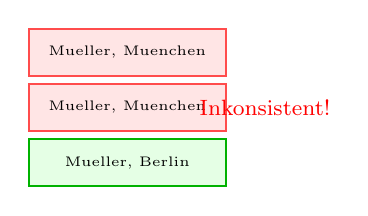
\begin{tikzpicture}[scale=0.7]
    \node[badbox, minimum width=2.5cm, font=\tiny] at (0,2) {Mueller, Muenchen};
    \node[badbox, minimum width=2.5cm, font=\tiny] at (0,1) {Mueller, Muenchen};
    \node[goodbox, minimum width=2.5cm, font=\tiny] at (0,0) {Mueller, Berlin};
    \node[font=\footnotesize, red] at (2.5,1) {Inkonsistent!};
\end{tikzpicture}
\end{center}
\small
Update vergessen $\rightarrow$ Widerspruch in den Daten

\column{0.33\textwidth}
\textbf{Einfuegeanomalie:}
\begin{center}
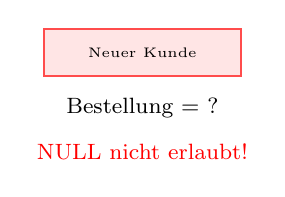
\begin{tikzpicture}[scale=0.7]
    \node[badbox, minimum width=2.5cm, font=\tiny] at (0,1.5) {Neuer Kunde};
    \node[font=\footnotesize] at (0,0.5) {Bestellung = ?};
    \node[font=\footnotesize, red] at (0,-0.3) {NULL nicht erlaubt!};
\end{tikzpicture}
\end{center}
\small
Neuer Kunde ohne Bestellung nicht speicherbar

\column{0.33\textwidth}
\textbf{Loeschanomalie:}
\begin{center}

\begin{tikzpicture}[scale=0.7]
    \node[badbox, minimum width=2.5cm, font=\tiny] at (0,1.5) {Letzte Bestellung};
    \node[font=\footnotesize] at (0,0.5) {von Schmidt};
    \draw[red, thick] (-1.2,1.2) -- (1.2,1.8);
    \node[font=\footnotesize, red] at (0,-0.3) {Kundendaten weg!};
\end{tikzpicture}
\end{center}
\small
Bestellung loeschen $\rightarrow$ Kundendaten verloren
\end{columns}

\vspace{1em}
\begin{alertblock}{Kernproblem}
Alle Anomalien entstehen durch \textbf{Redundanz} -- die gleiche Information an mehreren Stellen.
\end{alertblock}
\end{frame}

\begin{frame}{Weiteres Beispiel: Bibliothekssystem}
\begin{center}
\small
\textbf{Ausleihe\_Unnorm}
\begin{tabular}{|c|c|c|c|c|c|}
\hline
\rowcolor{IMSBlue!20}
\textbf{\underline{Ausleihe\_Nr}} & \textbf{Leser} & \textbf{L\_Adresse} & \textbf{Buch} & \textbf{Autor} & \textbf{Datum} \\
\hline
501 & Anna & Hauptstr. 1 & SQL Guide & Meier & 01.03.2026 \\
\hline
502 & Anna & Hauptstr. 1 & Python Basics & Schmidt & 05.03.2026 \\
\hline
503 & Ben & Bahnweg 7 & SQL Guide & Meier & 10.03.2026 \\
\hline
504 & Anna & Hauptstr. 1 & Java Kompakt & Mueller & 12.03.2026 \\
\hline
\end{tabular}
\end{center}

\vspace{1em}
\textbf{Identifizieren Sie die Redundanzen:}
\begin{itemize}
    \item Anna's Adresse erscheint \underline{\hspace{2cm}} mal
    \item Der Autor von ``SQL Guide'' erscheint \underline{\hspace{2cm}} mal
    \item Was passiert, wenn Anna umzieht?
    \item Was passiert, wenn wir die letzte Ausleihe von Ben loeschen?
\end{itemize}
\end{frame}

% ===== PHASE 2: Funktionale Abhaengigkeiten =====
\showagenda{2}

\begin{frame}{Funktionale Abhaengigkeit (FD)}
\begin{block}{Definition}
Ein Attribut B ist \textbf{funktional abhaengig} von A (geschrieben: \fd{A}{B}), wenn zu jedem Wert von A \textbf{genau ein} Wert von B gehoert.
\end{block}

\vspace{1em}
\textbf{Beispiele:}
\begin{itemize}
    \item \fd{Matrikelnr}{Studentenname} \quad {\color{green!70!black}\cmark}
    \item \fd{PLZ}{Ort} \quad {\color{green!70!black}\cmark} (in Deutschland)
    \item \fd{Ort}{PLZ} \quad {\color{red}\xmark} (Muenchen hat viele PLZ)
    \item \fd{ISBN}{Buchtitel} \quad {\color{green!70!black}\cmark}
\end{itemize}

\vspace{1em}
\begin{center}
\begin{tikzpicture}
    \node[fdbox] (a) at (0,0) {A};
    \node[fdbox] (b) at (3,0) {B};
    \draw[fdarrow] (a) -- (b) node[midway, above] {bestimmt};
\end{tikzpicture}

\vspace{0.5em}
\small
``Wenn ich A kenne, kenne ich auch B.''
\end{center}
\end{frame}

\begin{frame}{FD-Notation und Schreibweisen}
\textbf{Verschiedene Notationen (alle aequivalent):}

\vspace{1em}
\begin{center}
\begin{tabular}{|l|l|}
\hline
\rowcolor{IMSBlue!20}
\textbf{Schreibweise} & \textbf{Bedeutung} \\
\hline
\fd{A}{B} & A bestimmt B \\
\hline
A $\rightarrow$ B & A bestimmt B \\
\hline
B ist FD von A & B haengt funktional von A ab \\
\hline
\fd{A}{B, C} & A bestimmt sowohl B als auch C \\
\hline
\fd{A, B}{C} & Die Kombination von A und B bestimmt C \\
\hline
\end{tabular}
\end{center}

\vspace{1em}
\textbf{Wichtig:}
\begin{itemize}
    \item \fd{A}{B} bedeutet \textbf{nicht} \fd{B}{A}
    \item Der Pfeil zeigt die \textbf{Richtung} der Abhaengigkeit
    \item Die linke Seite heisst \textbf{Determinante}
\end{itemize}
\end{frame}

\begin{frame}{FDs in unserem Beispiel}
\begin{center}
\small
\textbf{Bestellung\_Unnorm}(\underline{Best\_Nr}, Kunde, K\_Stadt, Produkt, P\_Preis, Menge)
\end{center}

\vspace{1em}
\textbf{Funktionale Abhaengigkeiten:}
\begin{itemize}
    \item \fd{Best\_Nr, Produkt}{Menge} \quad (Schluessel!)
    \item \fd{Best\_Nr}{Kunde, K\_Stadt} \quad (Bestellung $\rightarrow$ Kunde)
    \item \fd{Kunde}{K\_Stadt} \quad (Kunde $\rightarrow$ Stadt)
    \item \fd{Produkt}{P\_Preis} \quad (Produkt $\rightarrow$ Preis)
\end{itemize}

\vspace{1em}
\begin{alertblock}{Problem}
Es gibt FDs, die \textbf{nicht vom gesamten Schluessel} abhaengen!\\
Das ist die Ursache fuer Redundanz.
\end{alertblock}
\end{frame}

\begin{frame}{Uebung: FDs identifizieren}
\begin{center}
\small
\textbf{Mitarbeiter}(\underline{MA\_Nr}, Name, Abteilung, Abt\_Leiter, Projekt, Stunden)
\begin{tabular}{|c|c|c|c|c|c|}
\hline
\rowcolor{IMSBlue!20}
\textbf{MA\_Nr} & \textbf{Name} & \textbf{Abteilung} & \textbf{Abt\_Leiter} & \textbf{Projekt} & \textbf{Stunden} \\
\hline
101 & Anna & IT & Dr. Weber & Portal & 20 \\
\hline
101 & Anna & IT & Dr. Weber & App & 15 \\
\hline
102 & Ben & HR & Dr. Klein & Portal & 30 \\
\hline
103 & Carla & IT & Dr. Weber & App & 25 \\
\hline
\end{tabular}
\end{center}

\vspace{1em}
\textbf{Welche FDs gibt es? (Ankreuzen)}
\begin{itemize}
    \item[$\square$] \fd{MA\_Nr}{Name}
    \item[$\square$] \fd{MA\_Nr}{Abteilung}
    \item[$\square$] \fd{Abteilung}{Abt\_Leiter}
    \item[$\square$] \fd{MA\_Nr, Projekt}{Stunden}
    \item[$\square$] \fd{Projekt}{Stunden}
\end{itemize}
\end{frame}

\begin{frame}{Loesung: FDs identifizieren}
\begin{center}
\small
\textbf{Mitarbeiter}(\underline{MA\_Nr, Projekt}, Name, Abteilung, Abt\_Leiter, Stunden)
\end{center}

\vspace{1em}
\textbf{Funktionale Abhaengigkeiten:}
\begin{itemize}
    \item[\cmark] \fd{MA\_Nr}{Name} -- Ein MA hat genau einen Namen
    \item[\cmark] \fd{MA\_Nr}{Abteilung} -- Ein MA ist in genau einer Abteilung
    \item[\cmark] \fd{Abteilung}{Abt\_Leiter} -- Jede Abteilung hat einen Leiter
    \item[\cmark] \fd{MA\_Nr, Projekt}{Stunden} -- Schluessel-FD
    \item[\xmark] \fd{Projekt}{Stunden} -- Falsch! Verschiedene MAs arbeiten unterschiedlich lange
\end{itemize}

\vspace{1em}
\begin{center}
\begin{tikzpicture}[scale=0.8]
    \node[fdbox, minimum width=3cm] (key) at (0,0) {MA\_Nr, Projekt};
    \node[fdbox] (std) at (5,0) {Stunden};
    \node[fdbox] (name) at (2,-1.5) {Name, Abteilung};
    \node[fdbox] (leiter) at (6,-1.5) {Abt\_Leiter};

    \draw[fdarrow] (key.east) -- (std.west);
    \draw[fdarrow, red] (key.south west) -- (name.north) node[midway, left, font=\footnotesize] {MA\_Nr};
    \draw[fdarrow, red] (name.east) -- (leiter.west) node[midway, above, font=\footnotesize] {Abt};
\end{tikzpicture}
\end{center}
\end{frame}

\begin{frame}{Volle vs. Partielle Abhaengigkeit}
\begin{columns}[T]
\column{0.5\textwidth}
\textbf{Volle funktionale Abhaengigkeit:}

B ist \textbf{voll} funktional abhaengig von A, wenn B von A abhaengt, aber \textbf{nicht} von einer echten Teilmenge von A.

\vspace{1em}
\textbf{Beispiel:}\\
\fd{Best\_Nr, Produkt}{Menge}

$\rightarrow$ Menge haengt vom \textbf{gesamten} Schluessel ab.

\column{0.5\textwidth}
\textbf{Partielle Abhaengigkeit:}

B haengt nur von einem \textbf{Teil} des Schluessels ab.

\vspace{1em}
\textbf{Beispiel:}\\
\fd{Best\_Nr}{Kunde}

$\rightarrow$ Kunde haengt nur von Best\_Nr ab, nicht von Produkt.

\vspace{1em}
{\color{red}\textbf{Das verursacht Redundanz!}}
\end{columns}

\vspace{1em}
\begin{center}
\begin{tikzpicture}
    \node[fdbox, minimum width=3cm] (key) at (0,0) {Best\_Nr, Produkt};
    \node[fdbox] (menge) at (4.5,0) {Menge};
    \node[fdbox] (kunde) at (4.5,-1.2) {Kunde};

    \draw[fdarrow] (key.east) -- (menge.west) node[midway, above, font=\footnotesize] {voll};
    \draw[fdarrow, red] (key.south) -- (kunde.west) node[midway, below, font=\footnotesize, sloped] {partiell};
    \node[font=\footnotesize, red] at (-0.8,-0.5) {Best\_Nr};
\end{tikzpicture}
\end{center}
\end{frame}

\begin{frame}{Armstrong's Axiome}
\textbf{Regeln zur Herleitung von FDs:}

\vspace{1em}
\begin{block}{1. Reflexivitaet}
Wenn B $\subseteq$ A, dann gilt \fd{A}{B}

\vspace{0.3em}
\small Beispiel: \fd{Vorname, Nachname}{Nachname}
\end{block}

\begin{block}{2. Augmentation (Erweiterung)}
Wenn \fd{A}{B}, dann gilt auch \fd{A, C}{B, C}

\vspace{0.3em}
\small Beispiel: Aus \fd{MA\_Nr}{Name} folgt \fd{MA\_Nr, Projekt}{Name, Projekt}
\end{block}

\begin{block}{3. Transitivitaet}
Wenn \fd{A}{B} und \fd{B}{C}, dann gilt \fd{A}{C}

\vspace{0.3em}
\small Beispiel: \fd{MA\_Nr}{Abteilung} und \fd{Abteilung}{Leiter} $\Rightarrow$ \fd{MA\_Nr}{Leiter}
\end{block}

\vspace{0.5em}
\textbf{Diese drei Axiome sind \textit{vollstaendig} -- alle ableitbaren FDs lassen sich damit herleiten!}
\end{frame}

\begin{frame}{Abgeleitete Regeln aus Armstrong's Axiomen}
\textbf{Nuetzliche Zusatzregeln (ableitbar aus den Axiomen):}

\vspace{1em}
\begin{columns}[T]
\column{0.5\textwidth}
\textbf{Vereinigung:}\\
Wenn \fd{A}{B} und \fd{A}{C},\\
dann \fd{A}{B, C}

\vspace{1em}
\textbf{Beispiel:}\\
\fd{ISBN}{Titel} und \fd{ISBN}{Autor}\\
$\Rightarrow$ \fd{ISBN}{Titel, Autor}

\column{0.5\textwidth}
\textbf{Dekomposition:}\\
Wenn \fd{A}{B, C},\\
dann \fd{A}{B} und \fd{A}{C}

\vspace{1em}
\textbf{Beispiel:}\\
\fd{MA\_Nr}{Name, Abteilung}\\
$\Rightarrow$ \fd{MA\_Nr}{Name} und \fd{MA\_Nr}{Abteilung}
\end{columns}

\vspace{1em}
\begin{alertblock}{Pseudotransitivitaet}
Wenn \fd{A}{B} und \fd{B, C}{D}, dann \fd{A, C}{D}
\end{alertblock}
\end{frame}

\begin{frame}{Quiz: Welche FDs sind ableitbar?}
\textbf{Gegeben:}
\begin{itemize}
    \item \fd{A}{B}
    \item \fd{B}{C}
    \item \fd{C, D}{E}
\end{itemize}

\vspace{1em}
\textbf{Welche FDs koennen abgeleitet werden?}

\vspace{0.5em}
\begin{tabular}{|l|c|l|}
\hline
\rowcolor{IMSBlue!20}
\textbf{FD} & \textbf{Ableitbar?} & \textbf{Begruendung} \\
\hline
\fd{A}{C} & \pause \cmark & Transitivitaet: A$\rightarrow$B$\rightarrow$C \\
\hline
\fd{A, D}{E} & \pause \cmark & Pseudotrans.: A$\rightarrow$C, CD$\rightarrow$E \\
\hline
\fd{B}{E} & \pause \xmark & D fehlt fuer C,D$\rightarrow$E \\
\hline
\fd{A}{B, C} & \pause \cmark & Vereinigung: A$\rightarrow$B, A$\rightarrow$C \\
\hline
\end{tabular}
\end{frame}

% ===== Hands-on: FDs =====
{
\setbeamercolor{background canvas}{bg=IMSOrange!15}
\begin{frame}[plain]
\vfill
\begin{center}
{\Huge\color{IMSOrange} Hands-on}\\[1em]
{\Large Funktionale Abhaengigkeiten erkennen}\\[2em]
{\large\ttfamily marimo: 08-normalisierung.py}\\[1em]
{\normalsize Aufgabe 8.1: FDs aus Beispieldaten ableiten}
\end{center}
\vfill
\end{frame}
}

% ===== PHASE 3: 1NF =====
\showagenda{3}

\begin{frame}{Erste Normalform (1NF)}
\begin{block}{Definition: 1NF}
Eine Relation ist in \textbf{1NF}, wenn alle Attributwerte \textbf{atomar} sind (keine Listen, keine geschachtelten Strukturen).
\end{block}

\vspace{1em}
\begin{columns}[T]
\column{0.5\textwidth}
\textbf{Nicht in 1NF:}
\begin{center}
\small
\begin{tabular}{|c|c|}
\hline
\rowcolor{red!20}
\textbf{Student} & \textbf{Kurse} \\
\hline
Anna & DMA, BWL, Statistik \\
\hline
Ben & DMA \\
\hline
\end{tabular}
\end{center}

{\color{red}\xmark} ``Kurse'' enthaelt eine \textbf{Liste}

\column{0.5\textwidth}
\textbf{In 1NF:}
\begin{center}
\small
\begin{tabular}{|c|c|}
\hline
\rowcolor{green!20}
\textbf{Student} & \textbf{Kurs} \\
\hline
Anna & DMA \\
\hline
Anna & BWL \\
\hline
Anna & Statistik \\
\hline
Ben & DMA \\
\hline
\end{tabular}
\end{center}

{\color{green!70!black}\cmark} Jede Zelle enthaelt \textbf{einen} Wert
\end{columns}

\vspace{1em}
\begin{alertblock}{Merke}
1NF ist die \textbf{Mindestanforderung} fuer relationale Datenbanken!
\end{alertblock}
\end{frame}

\begin{frame}{1NF-Verletzungen erkennen}
\textbf{Typische Anzeichen:}
\begin{itemize}
    \item Komma-separierte Werte: ``Muenchen, Berlin, Hamburg''
    \item Nummerierte Spalten: Telefon1, Telefon2, Telefon3
    \item JSON/XML in einer Spalte
    \item ``Wiederholungsgruppen''
\end{itemize}

\vspace{1em}
\textbf{Loesung:}
\begin{enumerate}
    \item Wiederholende Werte in \textbf{separate Zeilen} aufteilen
    \item Oder: \textbf{Neue Tabelle} erstellen (bei 1:N oder M:N)
\end{enumerate}

\vspace{1em}
\begin{exampleblock}{Beispiel: Telefonnummern}
\texttt{Person(ID, Name, Telefon1, Telefon2, Telefon3)}\\
$\downarrow$\\
\texttt{Person(ID, Name)} + \texttt{Telefon(\underline{Person\_ID, Nummer})}
\end{exampleblock}
\end{frame}

\begin{frame}{1NF: Schritt-fuer-Schritt Beispiel}
\textbf{Ausgangstabelle (nicht 1NF):}
\begin{center}
\small
\begin{tabular}{|c|c|c|}
\hline
\rowcolor{red!20}
\textbf{\underline{Kurs\_ID}} & \textbf{Kursname} & \textbf{Dozenten} \\
\hline
DMA01 & Datenmanagement & Flath, Mueller \\
\hline
BWL01 & Einfuehrung BWL & Schmidt \\
\hline
\end{tabular}
\end{center}

\vspace{1em}
\textbf{Schritt 1:} Wiederholende Werte identifizieren $\rightarrow$ ``Dozenten''

\vspace{0.5em}
\textbf{Schritt 2:} Aufteilen in atomare Werte:
\begin{center}
\small
\begin{tabular}{|c|c|c|}
\hline
\rowcolor{green!20}
\textbf{\underline{Kurs\_ID}} & \textbf{Kursname} & \textbf{\underline{Dozent}} \\
\hline
DMA01 & Datenmanagement & Flath \\
\hline
DMA01 & Datenmanagement & Mueller \\
\hline
BWL01 & Einfuehrung BWL & Schmidt \\
\hline
\end{tabular}
\end{center}

\vspace{0.5em}
\textbf{Hinweis:} Der Schluessel hat sich geaendert! Jetzt: (Kurs\_ID, Dozent)
\end{frame}

\begin{frame}{Quiz: Welche Tabelle ist in 1NF?}
\begin{columns}[T]
\column{0.5\textwidth}
\textbf{Tabelle A:}
\begin{center}
\footnotesize
\begin{tabular}{|c|c|c|}
\hline
\rowcolor{IMSBlue!20}
\textbf{ID} & \textbf{Name} & \textbf{Skills} \\
\hline
1 & Anna & Java, Python \\
\hline
2 & Ben & SQL \\
\hline
\end{tabular}
\end{center}

\vspace{2em}
\textbf{Tabelle B:}
\begin{center}
\footnotesize
\begin{tabular}{|c|c|c|}
\hline
\rowcolor{IMSBlue!20}
\textbf{ID} & \textbf{Name} & \textbf{Skill} \\
\hline
1 & Anna & Java \\
\hline
1 & Anna & Python \\
\hline
2 & Ben & SQL \\
\hline
\end{tabular}
\end{center}

\column{0.5\textwidth}
\textbf{Tabelle C:}
\begin{center}
\footnotesize
\begin{tabular}{|c|c|c|c|}
\hline
\rowcolor{IMSBlue!20}
\textbf{ID} & \textbf{Name} & \textbf{Skill1} & \textbf{Skill2} \\
\hline
1 & Anna & Java & Python \\
\hline
2 & Ben & SQL & NULL \\
\hline
\end{tabular}
\end{center}

\vspace{2em}
\textbf{Antwort:}\\[0.5em]
\pause
\begin{itemize}
    \item A: \xmark{} Liste in Zelle
    \item B: \cmark{} Atomar!
    \item C: \xmark{} Wiederholungsgruppe
\end{itemize}
\end{columns}
\end{frame}

% ===== PHASE 4: 2NF =====
\showagenda{4}

\begin{frame}{Zweite Normalform (2NF)}
\begin{block}{Definition: 2NF}
Eine Relation ist in \textbf{2NF}, wenn sie in 1NF ist und jedes Nicht-Schluesselattribut \textbf{voll funktional abhaengig} vom \textbf{gesamten} Primaerschluessel ist.
\end{block}

\vspace{1em}
\textbf{Anders gesagt:} Keine partiellen Abhaengigkeiten!

\vspace{1em}
\begin{center}
\begin{tikzpicture}
    \node[nfbox, fill=IMSBlue!10] (1nf) at (0,0) {1NF};
    \node[nfbox, fill=IMSBlue!20] (2nf) at (3.5,0) {2NF};
    \node[nfbox, fill=IMSBlue!30] (3nf) at (7,0) {3NF};

    \draw[roadmaparrow] (1nf.east) -- (2nf.west) node[midway, above, font=\footnotesize] {+ voll abhaengig};
    \draw[roadmaparrow] (2nf.east) -- (3nf.west) node[midway, above, font=\footnotesize] {+ nicht transitiv};
\end{tikzpicture}
\end{center}

\vspace{1em}
\begin{alertblock}{Wichtig}
2NF ist nur relevant bei \textbf{zusammengesetzten} Primaerschluesseln!\\
Bei einfachem PK ist eine 1NF-Relation automatisch in 2NF.
\end{alertblock}
\end{frame}

\begin{frame}{2NF-Verletzung erkennen}
\begin{center}
\small
\textbf{Bestellung\_Pos}(\underline{Best\_Nr, Produkt}, Kunde, K\_Stadt, P\_Preis, Menge)
\end{center}

\vspace{1em}
\textbf{Funktionale Abhaengigkeiten:}
\begin{itemize}
    \item \fd{Best\_Nr, Produkt}{Menge} \quad {\color{green!70!black}\cmark} voll abhaengig
    \item \fd{Best\_Nr}{Kunde, K\_Stadt} \quad {\color{red}\xmark} \textbf{partiell!}
    \item \fd{Produkt}{P\_Preis} \quad {\color{red}\xmark} \textbf{partiell!}
\end{itemize}

\vspace{1em}
\begin{center}
\begin{tikzpicture}[scale=0.9]
    \node[draw, rectangle, minimum width=4cm, minimum height=0.8cm] (key) at (0,0) {\underline{Best\_Nr, Produkt}};
    \node[draw, rectangle, fill=green!10] (menge) at (5.5,0) {Menge};
    \node[draw, rectangle, fill=red!10] (kunde) at (2.5,-1.8) {Kunde, K\_Stadt};
    \node[draw, rectangle, fill=red!10] (preis) at (7,-1.8) {P\_Preis};

    \draw[fdarrow, green!70!black] (key.east) -- (menge.west) node[midway, above, font=\footnotesize] {voll};
    \draw[fdarrow, red] ([xshift=-0.6cm]key.south) -- (kunde.north) node[midway, left, font=\footnotesize] {Best\_Nr};
    \draw[fdarrow, red] ([xshift=0.6cm]key.south) -- (preis.north) node[midway, right, font=\footnotesize] {Produkt};
\end{tikzpicture}
\end{center}
\end{frame}

\begin{frame}{2NF herstellen: Zerlegung}
\textbf{Loesung:} Attribute, die nur von einem Teil des Schluessels abhaengen, in \textbf{eigene Tabellen} auslagern.

\vspace{1em}
\begin{center}
\small
\textbf{Vorher (nicht 2NF):}\\
Bestellung\_Pos(\underline{Best\_Nr, Produkt}, Kunde, K\_Stadt, P\_Preis, Menge)

\vspace{1em}
$\Downarrow$ Zerlegung

\vspace{1em}
\textbf{Nachher (2NF):}\\
\texttt{Bestellung(\underline{Best\_Nr}, Kunde, K\_Stadt)}\\
\texttt{Produkt(\underline{Produkt}, P\_Preis)}\\
\texttt{Best\_Position(\underline{Best\_Nr, Produkt}, Menge)}
\end{center}

\vspace{1em}
\begin{block}{Ergebnis}
Jede Tabelle hat nur noch Attribute, die \textbf{voll} vom Schluessel abhaengen.
\end{block}
\end{frame}

\begin{frame}{2NF: Schritt-fuer-Schritt Walkthrough}
\textbf{Ausgangstabelle:} Vorlesung(\underline{VL\_Nr, Dozent\_ID}, VL\_Name, Raum, Dozent\_Name)

\vspace{0.5em}
\textbf{Schritt 1: FDs identifizieren}
\begin{itemize}
    \item \fd{VL\_Nr, Dozent\_ID}{Raum} -- voll (Dozent kann unterschiedliche Raeume haben)
    \item \fd{VL\_Nr}{VL\_Name} -- \textbf{partiell!}
    \item \fd{Dozent\_ID}{Dozent\_Name} -- \textbf{partiell!}
\end{itemize}

\vspace{0.5em}
\textbf{Schritt 2: Partielle FDs auslagern}
\begin{itemize}
    \item Neue Tabelle fuer \fd{VL\_Nr}{VL\_Name}
    \item Neue Tabelle fuer \fd{Dozent\_ID}{Dozent\_Name}
\end{itemize}

\vspace{0.5em}
\textbf{Schritt 3: Ergebnis (2NF)}
\begin{itemize}
    \item \texttt{Vorlesung(\underline{VL\_Nr}, VL\_Name)}
    \item \texttt{Dozent(\underline{Dozent\_ID}, Dozent\_Name)}
    \item \texttt{VL\_Dozent(\underline{VL\_Nr, Dozent\_ID}, Raum)}
\end{itemize}
\end{frame}

\begin{frame}{Haeufiger Fehler: 2NF bei einfachem Schluessel}
\begin{alertblock}{Achtung!}
Bei einem \textbf{einfachen} (nicht zusammengesetzten) Primaerschluessel gibt es \textbf{keine partiellen Abhaengigkeiten}.
\end{alertblock}

\vspace{1em}
\textbf{Beispiel:}\\
\texttt{Kunde(\underline{Kunden\_ID}, Name, Stadt, PLZ)}

\vspace{0.5em}
\begin{itemize}
    \item \fd{Kunden\_ID}{Name} -- voll (Schluessel hat nur 1 Attribut)
    \item \fd{Kunden\_ID}{Stadt} -- voll
    \item \fd{Kunden\_ID}{PLZ} -- voll
\end{itemize}

\vspace{1em}
$\Rightarrow$ Diese Relation ist \textbf{automatisch in 2NF}!

\vspace{1em}
\textbf{Aber:} Es koennte trotzdem eine 3NF-Verletzung geben (transitive Abhaengigkeit: \fd{PLZ}{Stadt})
\end{frame}

\begin{frame}{Quiz: Welche NF?}
\textbf{Gegeben:} Buchung(\underline{Hotel\_ID, Gast\_ID, Datum}, Zimmer, Hotel\_Name, Gast\_Name)

\vspace{1em}
\textbf{FDs:}
\begin{itemize}
    \item \fd{Hotel\_ID, Gast\_ID, Datum}{Zimmer}
    \item \fd{Hotel\_ID}{Hotel\_Name}
    \item \fd{Gast\_ID}{Gast\_Name}
\end{itemize}

\vspace{1em}
\textbf{In welcher Normalform ist die Relation?}

\vspace{0.5em}
\begin{enumerate}
    \item[A)] Nicht in 1NF
    \item[B)] In 1NF, aber nicht 2NF
    \item[C)] In 2NF, aber nicht 3NF
    \item[D)] In 3NF
\end{enumerate}

\pause
\vspace{0.5em}
\textbf{Antwort: B)} -- Partielle Abhaengigkeiten vorhanden (Hotel\_Name, Gast\_Name)
\end{frame}

% ===== Hands-on =====
{
\setbeamercolor{background canvas}{bg=IMSOrange!15}
\begin{frame}[plain]
\vfill
\begin{center}
{\Huge\color{IMSOrange} Hands-on}\\[1em]
{\Large 1NF und 2NF anwenden}\\[2em]
{\large\ttfamily marimo: 08-normalisierung.py}\\[1em]
{\normalsize Aufgaben 8.2 -- 8.3}
\end{center}
\vfill
\end{frame}
}

% ===== PAUSE =====
\begin{frame}[plain]
\vfill
\begin{center}
{\Huge Pause}\\[1em]
{\LARGE 15 Minuten}\\[0.5em]
{\large Kaffee holen!}
\end{center}
\vfill
\end{frame}

% ===== PHASE 5: 3NF =====
\showagenda{5}

\begin{frame}{Dritte Normalform (3NF)}
\begin{block}{Definition: 3NF}
Eine Relation ist in \textbf{3NF}, wenn sie in 2NF ist und kein Nicht-Schluesselattribut \textbf{transitiv} vom Primaerschluessel abhaengt.
\end{block}

\vspace{1em}
\textbf{Transitive Abhaengigkeit:}\\
\fd{A}{B} und \fd{B}{C} $\Rightarrow$ C haengt \textbf{transitiv} von A ab.

\vspace{1em}
\begin{center}
\begin{tikzpicture}
    \node[fdbox] (a) at (0,0) {A (PK)};
    \node[fdbox] (b) at (3,0) {B};
    \node[fdbox] (c) at (6,0) {C};

    \draw[fdarrow] (a) -- (b);
    \draw[fdarrow] (b) -- (c);
    \draw[fdarrow, dashed, red, bend left=30] (a) to node[above, font=\footnotesize] {transitiv!} (c);
\end{tikzpicture}
\end{center}

\vspace{1em}
\textbf{Problem:} C ist redundant gespeichert -- wenn B sich wiederholt, wird auch C wiederholt!
\end{frame}

\begin{frame}{3NF-Verletzung erkennen}
\begin{center}
\small
\textbf{Bestellung}(\underline{Best\_Nr}, Kunde, K\_Stadt)
\end{center}

\vspace{1em}
\textbf{Funktionale Abhaengigkeiten:}
\begin{itemize}
    \item \fd{Best\_Nr}{Kunde} \quad {\color{green!70!black}\cmark}
    \item \fd{Kunde}{K\_Stadt} \quad (Kunde bestimmt Stadt)
    \item $\Rightarrow$ \fd{Best\_Nr}{K\_Stadt} \quad {\color{red}\xmark} \textbf{transitiv!}
\end{itemize}

\vspace{1em}
\begin{center}
\begin{tikzpicture}
    \node[fdbox] (bestnr) at (0,0) {\underline{Best\_Nr}};
    \node[fdbox] (kunde) at (3,0) {Kunde};
    \node[fdbox, fill=red!10] (stadt) at (6,0) {K\_Stadt};

    \draw[fdarrow] (bestnr) -- (kunde);
    \draw[fdarrow] (kunde) -- (stadt);
    \draw[fdarrow, dashed, red, bend left=30] (bestnr) to (stadt);
\end{tikzpicture}
\end{center}

\vspace{1em}
\textbf{Redundanz:} Wenn Mueller 5 Bestellungen hat, steht ``Muenchen'' 5x in der Tabelle.
\end{frame}

\begin{frame}{3NF herstellen: Zerlegung}
\textbf{Loesung:} Die transitive Abhaengigkeit in eine \textbf{eigene Tabelle} auslagern.

\vspace{1em}
\begin{center}
\small
\textbf{Vorher (nicht 3NF):}\\
Bestellung(\underline{Best\_Nr}, Kunde, K\_Stadt)

\vspace{1em}
$\Downarrow$ Zerlegung

\vspace{1em}
\textbf{Nachher (3NF):}\\
\texttt{Bestellung(\underline{Best\_Nr}, \#Kunde)}\\
\texttt{Kunde(\underline{Kunde}, K\_Stadt)}
\end{center}

\vspace{1em}
\begin{block}{Ergebnis}
Jedes Nicht-Schluesselattribut haengt \textbf{direkt} (nicht transitiv) vom Schluessel ab.
\end{block}
\end{frame}

\begin{frame}{3NF: Schritt-fuer-Schritt Walkthrough}
\textbf{Ausgangstabelle (2NF):} Mitarbeiter(\underline{MA\_Nr}, Name, Abt\_ID, Abt\_Name, Abt\_Ort)

\vspace{0.5em}
\textbf{Schritt 1: Transitive FDs finden}
\begin{itemize}
    \item \fd{MA\_Nr}{Abt\_ID} -- direkt
    \item \fd{Abt\_ID}{Abt\_Name} -- nicht vom PK!
    \item \fd{Abt\_ID}{Abt\_Ort} -- nicht vom PK!
    \item $\Rightarrow$ \fd{MA\_Nr}{Abt\_Name} -- \textbf{transitiv!}
    \item $\Rightarrow$ \fd{MA\_Nr}{Abt\_Ort} -- \textbf{transitiv!}
\end{itemize}

\vspace{0.5em}
\textbf{Schritt 2: Transitive Attribute auslagern}

\vspace{0.5em}
\textbf{Schritt 3: Ergebnis (3NF)}
\begin{itemize}
    \item \texttt{Mitarbeiter(\underline{MA\_Nr}, Name, \#Abt\_ID)}
    \item \texttt{Abteilung(\underline{Abt\_ID}, Abt\_Name, Abt\_Ort)}
\end{itemize}
\end{frame}

\begin{frame}{Beispiel: Universitaetssystem}
\textbf{Ausgangstabelle:}\\
\small Einschreibung(\underline{Matrikel}, Student\_Name, \underline{Kurs\_ID}, Kurs\_Name, Dozent\_ID, Dozent\_Name, Note)

\vspace{0.5em}
\textbf{FDs:}
\begin{itemize}
    \item \fd{Matrikel}{Student\_Name}
    \item \fd{Kurs\_ID}{Kurs\_Name, Dozent\_ID}
    \item \fd{Dozent\_ID}{Dozent\_Name}
    \item \fd{Matrikel, Kurs\_ID}{Note}
\end{itemize}

\vspace{0.5em}
\textbf{Probleme:}
\begin{itemize}
    \item Partielle Abhaengigkeit: Student\_Name von Matrikel (nicht 2NF)
    \item Partielle Abhaengigkeit: Kurs\_Name, Dozent\_ID von Kurs\_ID (nicht 2NF)
    \item Transitive Abhaengigkeit: Dozent\_Name ueber Dozent\_ID (nicht 3NF)
\end{itemize}
\end{frame}

\begin{frame}{Beispiel: Universitaetssystem -- Loesung}
\textbf{Normalisierte Tabellen (3NF):}

\vspace{1em}
\begin{center}
\begin{tikzpicture}[scale=0.85, every node/.style={scale=0.85}]
    \node[goodbox, minimum width=5cm] (stud) at (-3,2) {Student(\underline{Matrikel}, Name)};
    \node[goodbox, minimum width=5cm] (kurs) at (3,2) {Kurs(\underline{Kurs\_ID}, Name, \#Doz\_ID)};
    \node[goodbox, minimum width=5cm] (doz) at (3,0) {Dozent(\underline{Doz\_ID}, Name)};
    \node[goodbox, minimum width=6cm] (einschr) at (0,-1.5) {Einschreibung(\underline{Matrikel, Kurs\_ID}, Note)};

    \draw[roadmaparrow] (stud.south) -- (einschr.north west);
    \draw[roadmaparrow] (kurs.south west) -- (einschr.north east);
    \draw[roadmaparrow] (doz.west) -- (kurs.south);
\end{tikzpicture}
\end{center}

\vspace{1em}
\textbf{Vorteile:}
\begin{itemize}
    \item Studentendaten nur einmal gespeichert
    \item Kursdaten nur einmal gespeichert
    \item Dozentendaten nur einmal gespeichert
    \item Keine Anomalien mehr moeglich!
\end{itemize}
\end{frame}

\begin{frame}{Vollstaendige Normalisierung: Beispiel}
\begin{center}
\textbf{Ausgangstabelle (nicht normalisiert):}\\[0.5em]
\small
Bestellung\_Unnorm(\underline{Best\_Nr}, Kunde, K\_Stadt, Produkt, P\_Preis, Menge)
\end{center}

\vspace{1em}
\begin{center}
\begin{tikzpicture}[node distance=0.8cm]
    \node[badbox, minimum width=8cm] (orig) {Best\_Nr, Kunde, K\_Stadt, Produkt, P\_Preis, Menge};

    \node[goodbox, below left=1.5cm and -1cm of orig] (best) {Bestellung(\underline{Best\_Nr}, \#Kunde)};
    \node[goodbox, below=1.5cm of orig] (kunde) {Kunde(\underline{Kunde}, K\_Stadt)};
    \node[goodbox, below right=1.5cm and -1cm of orig] (prod) {Produkt(\underline{Produkt}, P\_Preis)};
    \node[goodbox, below=3cm of orig] (pos) {Best\_Pos(\underline{Best\_Nr, Produkt}, Menge)};

    \draw[roadmaparrow] (orig) -- (best);
    \draw[roadmaparrow] (orig) -- (kunde);
    \draw[roadmaparrow] (orig) -- (prod);
    \draw[roadmaparrow] (orig) -- (pos);
\end{tikzpicture}
\end{center}

\vspace{0.5em}
\textbf{Ergebnis: 4 Tabellen in 3NF} -- keine Redundanz, keine Anomalien!
\end{frame}

\begin{frame}{Quiz: Welche Normalform?}
\textbf{Bewerten Sie jede Relation:}

\vspace{1em}
\begin{tabular}{|l|c|}
\hline
\rowcolor{IMSBlue!20}
\textbf{Relation} & \textbf{NF?} \\
\hline
Film(\underline{ID}, Titel, Regisseur, Genre, Genre\_Beschreibung) & \pause nicht 3NF \\
\hline
Buch(\underline{ISBN}, Titel, Autor1, Autor2, Autor3) & \pause nicht 1NF \\
\hline
Bestellung(\underline{Best\_Nr, Artikel}, Preis, Menge, Kunde\_Name) & \pause nicht 2NF \\
\hline
Mitarbeiter(\underline{MA\_ID}, Name, Gehalt) & \pause 3NF \\
\hline
\end{tabular}

\vspace{1em}
\textbf{Erklaerungen:}
\begin{itemize}
    \item Film: \fd{Genre}{Genre\_Beschreibung} ist transitiv
    \item Buch: Wiederholungsgruppe (mehrere Autor-Spalten)
    \item Bestellung: Preis haengt nur von Artikel ab (partiell)
    \item Mitarbeiter: Alle Attribute haengen direkt vom Schluessel ab
\end{itemize}
\end{frame}

\begin{frame}{Haeufige Fehler bei der Normalisierung}
\begin{columns}[T]
\column{0.5\textwidth}
\textbf{Fehler 1: FDs uebersehen}
\begin{itemize}
    \item Alle Geschaeftsregeln beachten!
    \item ``Jeder Kunde hat genau eine Adresse'' $\rightarrow$ FD
\end{itemize}

\vspace{1em}
\textbf{Fehler 2: Schluessel falsch bestimmt}
\begin{itemize}
    \item Schluessel muss minimal sein
    \item Alle Attribute bestimmen
\end{itemize}

\column{0.5\textwidth}
\textbf{Fehler 3: Zu frueh aufhoeren}
\begin{itemize}
    \item 2NF reicht nicht!
    \item Transitive FDs pruefen
\end{itemize}

\vspace{1em}
\textbf{Fehler 4: Zu viel zerlegen}
\begin{itemize}
    \item Nur bei echten Verletzungen zerlegen
    \item JOINs kosten Performance
\end{itemize}
\end{columns}

\vspace{1em}
\begin{alertblock}{Tipp}
Bei Unsicherheit: Beispieldaten durchspielen! Tritt Redundanz auf?
\end{alertblock}
\end{frame}

% ===== PHASE 6: BCNF & Denormalisierung =====
\showagenda{6}

\begin{frame}{Boyce-Codd-Normalform (BCNF)}
\begin{block}{Definition: BCNF}
Eine Relation ist in \textbf{BCNF}, wenn fuer jede nicht-triviale FD \fd{X}{Y} gilt: X ist ein \textbf{Superschluessel}.
\end{block}

\vspace{1em}
\textbf{BCNF ist strenger als 3NF:}
\begin{itemize}
    \item 3NF erlaubt: Schluesselattribut haengt von Nicht-Schluessel ab
    \item BCNF verbietet das
\end{itemize}

\vspace{1em}
\textbf{In der Praxis:}
\begin{itemize}
    \item Die meisten 3NF-Relationen sind auch BCNF
    \item BCNF kann manchmal nicht verlustfrei erreicht werden
    \item Fuer Klausuren: 3NF reicht meist!
\end{itemize}

\vspace{1em}
\begin{alertblock}{Merksatz}
``Jedes Attribut haengt vom Schluessel ab, vom ganzen Schluessel, und von nichts ausser dem Schluessel.'' (Codd)
\end{alertblock}
\end{frame}

\begin{frame}{3NF vs. BCNF: Der Unterschied}
\textbf{Beispiel:} Kurs(\underline{Student, Fach}, Dozent)

\vspace{0.5em}
\textbf{FDs:}
\begin{itemize}
    \item \fd{Student, Fach}{Dozent} -- Schluessel-FD
    \item \fd{Dozent}{Fach} -- Jeder Dozent unterrichtet nur ein Fach
\end{itemize}

\vspace{1em}
\textbf{3NF-Pruefung:}
\begin{itemize}
    \item Keine partiellen Abhaengigkeiten (Dozent haengt vom ganzen Schluessel ab)
    \item Keine transitiven Abhaengigkeiten (Dozent ist kein Nicht-Schluesselattribut in der zweiten FD)
    \item $\Rightarrow$ \cmark{} Ist in 3NF!
\end{itemize}

\vspace{0.5em}
\textbf{BCNF-Pruefung:}
\begin{itemize}
    \item \fd{Dozent}{Fach} -- Dozent ist kein Superschluessel!
    \item $\Rightarrow$ \xmark{} Ist NICHT in BCNF!
\end{itemize}
\end{frame}

\begin{frame}{Normalformen: Uebersicht}
\begin{center}
\begin{tikzpicture}[scale=0.9]
    % Nested boxes showing NF hierarchy (BCNF ⊂ 3NF ⊂ 2NF ⊂ 1NF)
    \draw[very thick, rounded corners=8pt, fill=gray!10, draw=gray!50] (-4,-2.5) rectangle (4,2.5);
    \node[font=\bfseries] at (3.2,2.2) {1NF};
    \node[font=\footnotesize, gray] at (0,-2.2) {Atomare Werte};

    \draw[very thick, rounded corners=6pt, fill=IMSBlue!10, draw=IMSBlue!50] (-3.3,-1.9) rectangle (3.3,1.9);
    \node[font=\bfseries] at (2.5,1.6) {2NF};
    \node[font=\footnotesize, IMSBlue!70] at (0,-1.6) {+ Keine partiellen FDs};

    \draw[very thick, rounded corners=4pt, fill=IMSBlue!20, draw=IMSBlue!70] (-2.5,-1.2) rectangle (2.5,1.2);
    \node[font=\bfseries] at (1.8,0.9) {3NF};
    \node[font=\footnotesize, IMSBlue] at (0,-0.9) {+ Keine transitiven FDs};

    \draw[very thick, rounded corners=2pt, fill=IMSBlue!35, draw=IMSBlue] (-1.6,-0.5) rectangle (1.6,0.5);
    \node[font=\bfseries] at (0,0) {BCNF};
\end{tikzpicture}
\end{center}

\vspace{1em}
\begin{center}
\begin{tabular}{|l|l|}
\hline
\rowcolor{IMSBlue!20}
\textbf{Normalform} & \textbf{Anforderung} \\
\hline
1NF & Atomare Werte \\
\hline
2NF & + Keine partiellen Abhaengigkeiten \\
\hline
3NF & + Keine transitiven Abhaengigkeiten \\
\hline
BCNF & + Jede Determinante ist Superschluessel \\
\hline
\end{tabular}
\end{center}
\end{frame}

\begin{frame}{Checkliste: Normalform bestimmen}
\textbf{Systematisches Vorgehen:}

\vspace{1em}
\begin{enumerate}
    \item \textbf{1NF pruefen:}
    \begin{itemize}
        \item Sind alle Werte atomar? (Keine Listen, keine Wiederholungsgruppen)
    \end{itemize}

    \vspace{0.5em}
    \item \textbf{Schluessel bestimmen:}
    \begin{itemize}
        \item Welche Attributkombination bestimmt alle anderen?
    \end{itemize}

    \vspace{0.5em}
    \item \textbf{2NF pruefen:} (nur bei zusammengesetztem Schluessel)
    \begin{itemize}
        \item Haengen alle Nicht-Schluesselattribute vom \textit{ganzen} Schluessel ab?
    \end{itemize}

    \vspace{0.5em}
    \item \textbf{3NF pruefen:}
    \begin{itemize}
        \item Gibt es FDs zwischen Nicht-Schluesselattributen?
        \item Falls ja: transitive Abhaengigkeit!
    \end{itemize}
\end{enumerate}
\end{frame}

\begin{frame}{Denormalisierung: Wann und Warum?}
\textbf{Normalisierung hat auch Nachteile:}
\begin{itemize}
    \item Viele Tabellen $\rightarrow$ viele JOINs noetig
    \item JOINs koennen \textbf{Performance kosten}
    \item Komplexere Abfragen
\end{itemize}

\vspace{1em}
\textbf{Denormalisierung = bewusste Einfuehrung von Redundanz}

\vspace{1em}
\textbf{Wann sinnvoll?}
\begin{itemize}
    \item Lesende Zugriffe dominieren (wenig Updates)
    \item Performance kritisch (z.B. Reporting, Data Warehouse)
    \item Daten aendern sich selten
\end{itemize}

\vspace{1em}
\begin{alertblock}{Wichtig}
Denormalisierung ist eine \textbf{bewusste Entscheidung} nach Abwaegung!\\
Erst normalisieren, dann gezielt denormalisieren.
\end{alertblock}
\end{frame}

\begin{frame}{Denormalisierung: Beispiele}
\textbf{Typische Denormalisierungsstrategien:}

\vspace{1em}
\begin{columns}[T]
\column{0.5\textwidth}
\textbf{1. Berechnete Spalten speichern:}
\begin{itemize}
    \item Statt: SUM(Positionen) bei jeder Abfrage
    \item Speichern: Bestellung.Gesamtsumme
    \item Vorteil: Schneller Zugriff
    \item Nachteil: Bei Aenderung nachfuehren
\end{itemize}

\column{0.5\textwidth}
\textbf{2. Haeufige JOINs vorwegnehmen:}
\begin{itemize}
    \item Statt: Bestellung JOIN Kunde
    \item Speichern: Kundenname in Bestellung
    \item Vorteil: Kein JOIN noetig
    \item Nachteil: Redundanz
\end{itemize}
\end{columns}

\vspace{1em}
\begin{exampleblock}{Data Warehouse}
In analytischen Systemen (OLAP) ist Denormalisierung Standard!\\
$\rightarrow$ ``Star Schema'', ``Snowflake Schema''
\end{exampleblock}
\end{frame}

\begin{frame}{Wann welche Normalform?}
\begin{center}
\begin{tabular}{|l|l|l|}
\hline
\rowcolor{IMSBlue!20}
\textbf{Situation} & \textbf{Empfehlung} & \textbf{Grund} \\
\hline
OLTP-System & 3NF (mindestens) & Datenintegritaet \\
\hline
Data Warehouse & 1NF/2NF & Leseperformance \\
\hline
Reporting-DB & Denormalisiert & Schnelle Abfragen \\
\hline
Stammdaten & 3NF/BCNF & Wenig Aenderungen \\
\hline
Bewegungsdaten & 3NF & Viele Aenderungen \\
\hline
\end{tabular}
\end{center}

\vspace{1em}
\textbf{Faustregel:}
\begin{itemize}
    \item \textbf{Viele Schreibzugriffe} $\rightarrow$ Hohe Normalform (3NF)
    \item \textbf{Viele Lesezugriffe} $\rightarrow$ Ggf. denormalisieren
    \item \textbf{Im Zweifel:} Erst normalisieren, dann messen, dann optimieren
\end{itemize}
\end{frame}

% ===== Hands-on =====
{
\setbeamercolor{background canvas}{bg=IMSOrange!15}
\begin{frame}[plain]
\vfill
\begin{center}
{\Huge\color{IMSOrange} Hands-on}\\[1em]
{\Large 3NF-Normalisierung durchfuehren}\\[2em]
{\large\ttfamily marimo: 08-normalisierung.py}\\[1em]
{\normalsize Aufgaben 8.4 -- 8.5}
\end{center}
\vfill
\end{frame}
}

% ===== PHASE 7: Zusammenfassung =====
\showagenda{7}

\begin{frame}{Zusammenfassung}
\begin{columns}[T]
\column{0.5\textwidth}
\textbf{Funktionale Abhaengigkeit:}
\begin{itemize}
    \item \fd{A}{B} = A bestimmt B
    \item Voll vs. partiell
    \item Transitiv: A$\rightarrow$B$\rightarrow$C
\end{itemize}

\vspace{1em}
\textbf{Normalformen:}
\begin{itemize}
    \item 1NF: Atomare Werte
    \item 2NF: Keine partiellen Abhaengigkeiten
    \item 3NF: Keine transitiven Abhaengigkeiten
\end{itemize}

\column{0.5\textwidth}
\textbf{Normalisierungsalgorithmus:}
\begin{enumerate}
    \item FDs identifizieren
    \item Schluessel bestimmen
    \item Verletzungen finden
    \item Tabelle zerlegen
    \item Wiederholen bis 3NF
\end{enumerate}

\vspace{1em}
\textbf{Denormalisierung:}
\begin{itemize}
    \item Bewusst Redundanz einfuehren
    \item Fuer Performance
    \item Nach Abwaegung!
\end{itemize}
\end{columns}
\end{frame}

\begin{frame}{Normalisierung: Der Algorithmus}
\begin{center}
\begin{tikzpicture}[node distance=1.2cm, scale=0.9, every node/.style={scale=0.9}]
    \node[roadmapbox, minimum width=6cm] (start) {Ausgangstabelle};
    \node[roadmapbox, minimum width=6cm, below=of start] (fd) {1. FDs identifizieren};
    \node[roadmapbox, minimum width=6cm, below=of fd] (key) {2. Schluessel bestimmen};
    \node[roadmapbox, minimum width=6cm, below=of key, fill=IMSOrange!10, draw=IMSOrange] (check) {3. NF-Verletzung?};
    \node[roadmapbox, minimum width=6cm, below=of check] (split) {4. Zerlegen};
    \node[roadmapbox, minimum width=6cm, fill=green!20, draw=green!50!black, below=of split] (done) {3NF erreicht!};

    \draw[roadmaparrow] (start) -- (fd);
    \draw[roadmaparrow] (fd) -- (key);
    \draw[roadmaparrow] (key) -- (check);
    \draw[roadmaparrow] (check) -- (split) node[midway, right, font=\small] {Ja};
    \draw[roadmaparrow, IMSOrange] (split.west) -- ++(-1.8,0) |- (check.west) node[pos=0.25, left, font=\small] {Wiederholen};
    \draw[roadmaparrow, green!50!black] (check.east) -- ++(1.8,0) |- (done.east) node[pos=0.25, right, font=\small] {Nein};
\end{tikzpicture}
\end{center}
\end{frame}

\begin{frame}{Cheat Sheet: Normalformen}
\begin{center}
\footnotesize
\begin{tabular}{|p{1.5cm}|p{4cm}|p{4cm}|p{3cm}|}
\hline
\rowcolor{IMSBlue!20}
\textbf{NF} & \textbf{Anforderung} & \textbf{Prueffrage} & \textbf{Loesung} \\
\hline
\textbf{1NF} & Atomare Werte & Listen in Zellen? Wiederholungsgruppen? & Aufteilen in Zeilen/Tabellen \\
\hline
\textbf{2NF} & Voll abhaengig vom PK & Haengt Attribut von Teil des Schluessels ab? & Teil-FD auslagern \\
\hline
\textbf{3NF} & Keine transitive FD & FD zwischen Nicht-Schluessel-Attributen? & Transitive FD auslagern \\
\hline
\textbf{BCNF} & Determinante = Superschluessel & Determinante kein Schluessel? & Auslagern \\
\hline
\end{tabular}
\end{center}

\vspace{1em}
\textbf{Merksatz (Codd):}
\begin{quote}
``Jedes Attribut haengt ab vom Schluessel, vom ganzen Schluessel, und von nichts ausser dem Schluessel -- so wahr mir Codd helfe!''
\end{quote}
\end{frame}

\begin{frame}{Ausblick: Naechste Session}
\textbf{Vorlesung 9: Joins}

\vspace{1em}
\begin{itemize}
    \item Daten aus mehreren Tabellen verknuepfen
    \item INNER JOIN, LEFT JOIN, RIGHT JOIN
    \item Self-Joins
    \item Join-Performance
\end{itemize}

\vspace{2em}
\begin{center}
\begin{tikzpicture}
    \node[roadmapbox] (norm) at (0,0) {Normalisierte Tabellen};
    \node[roadmapbox, fill=IMSOrange!20, draw=IMSOrange] (join) at (6,0) {JOIN};
    \draw[roadmaparrow] (norm) -- (join) node[midway, above] {verbinden};
\end{tikzpicture}
\end{center}

\vspace{1em}
\textbf{Jetzt haben wir gute Tabellen -- in Session 9 lernen wir, sie wieder zusammenzufuehren!}
\end{frame}

\begin{frame}[plain]
\vfill
\begin{center}
{\Huge Fragen?}\\[2em]
{\large christoph.flath@uni-wuerzburg.de}
\end{center}
\vfill
\end{frame}

\end{document}
